\chapter{Results}

\begin{comment}
Chapter 5: Results
Results that illustrate how the system designed by you works in practice, and how it is intended to be used, may be presented in this chapter. Screen shots may be useful to illustrate how the software interacts with the user.
\end{comment}

\plan{Print Screen Step Through of the Main Stuff the Application Does}

\section{System Walk-through}

\section{Responsive Web Design}

A key feature of the application is being able to access it at any time from any device, particularly when taking into account the rapid increase in the use of mobile devices.  Interacting with a website on a smartphone or tablet is not the same as interacting using a computer, due to the smaller screen size and use of touch over a mouse.

Forbes reported that 24\% of their 2013 website visits came from mobiles and 13\% from tablets, down from a total of 15\% in 2012. particularly with the high percentage of website visits coming from mobile devices \parencite{steimle2013responsive}.

In order to ensure the project is accessible from a variety of different devices the core UI uses Responsive Web Design (RWD) to layout the website differently depending on the size of the device to ensure an optimal viewing experience.

The differences depending on the device are highlighted in Figs. \ref{fig:responsive-macbook}-\ref{fig:responsive-iphone}.

\begin{figure}[h]
    \centering
    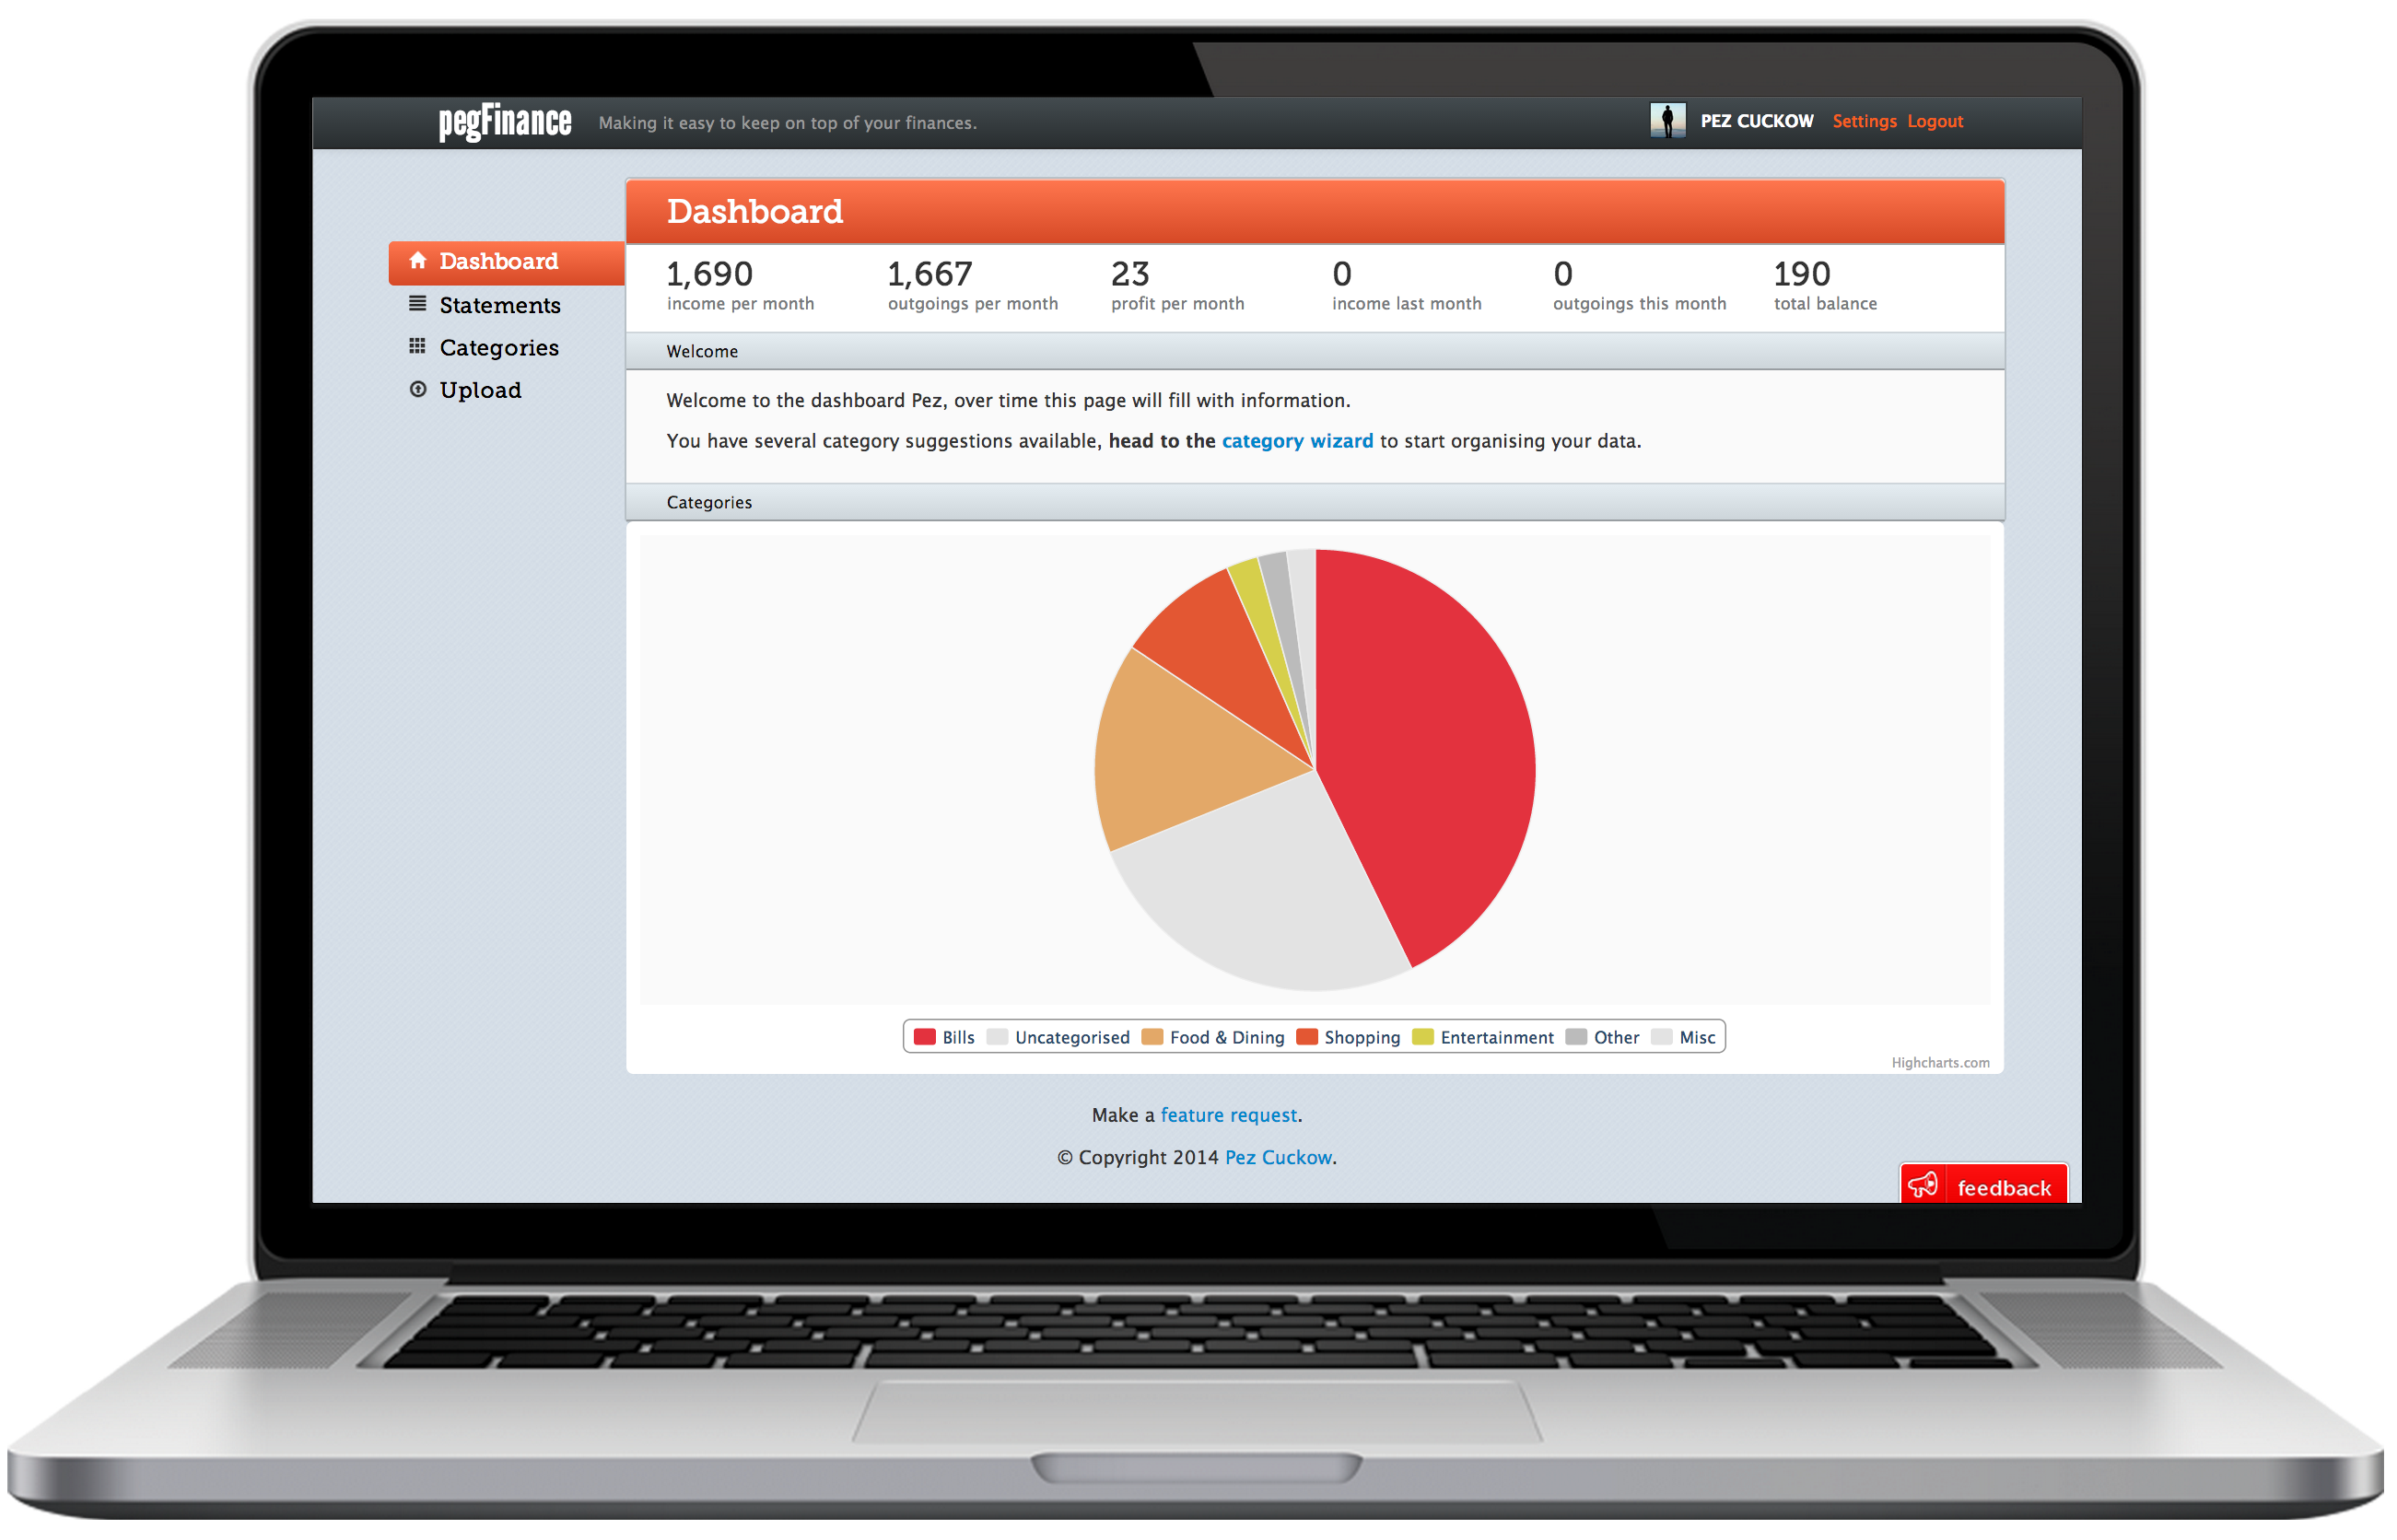
\includegraphics[width=0.8\textwidth]{screenshots/responsive/macbook}
    \caption{Layout on a standard laptop}
    \label{fig:responsive-macbook}
\end{figure}

\begin{figure}[h]
    \centering
    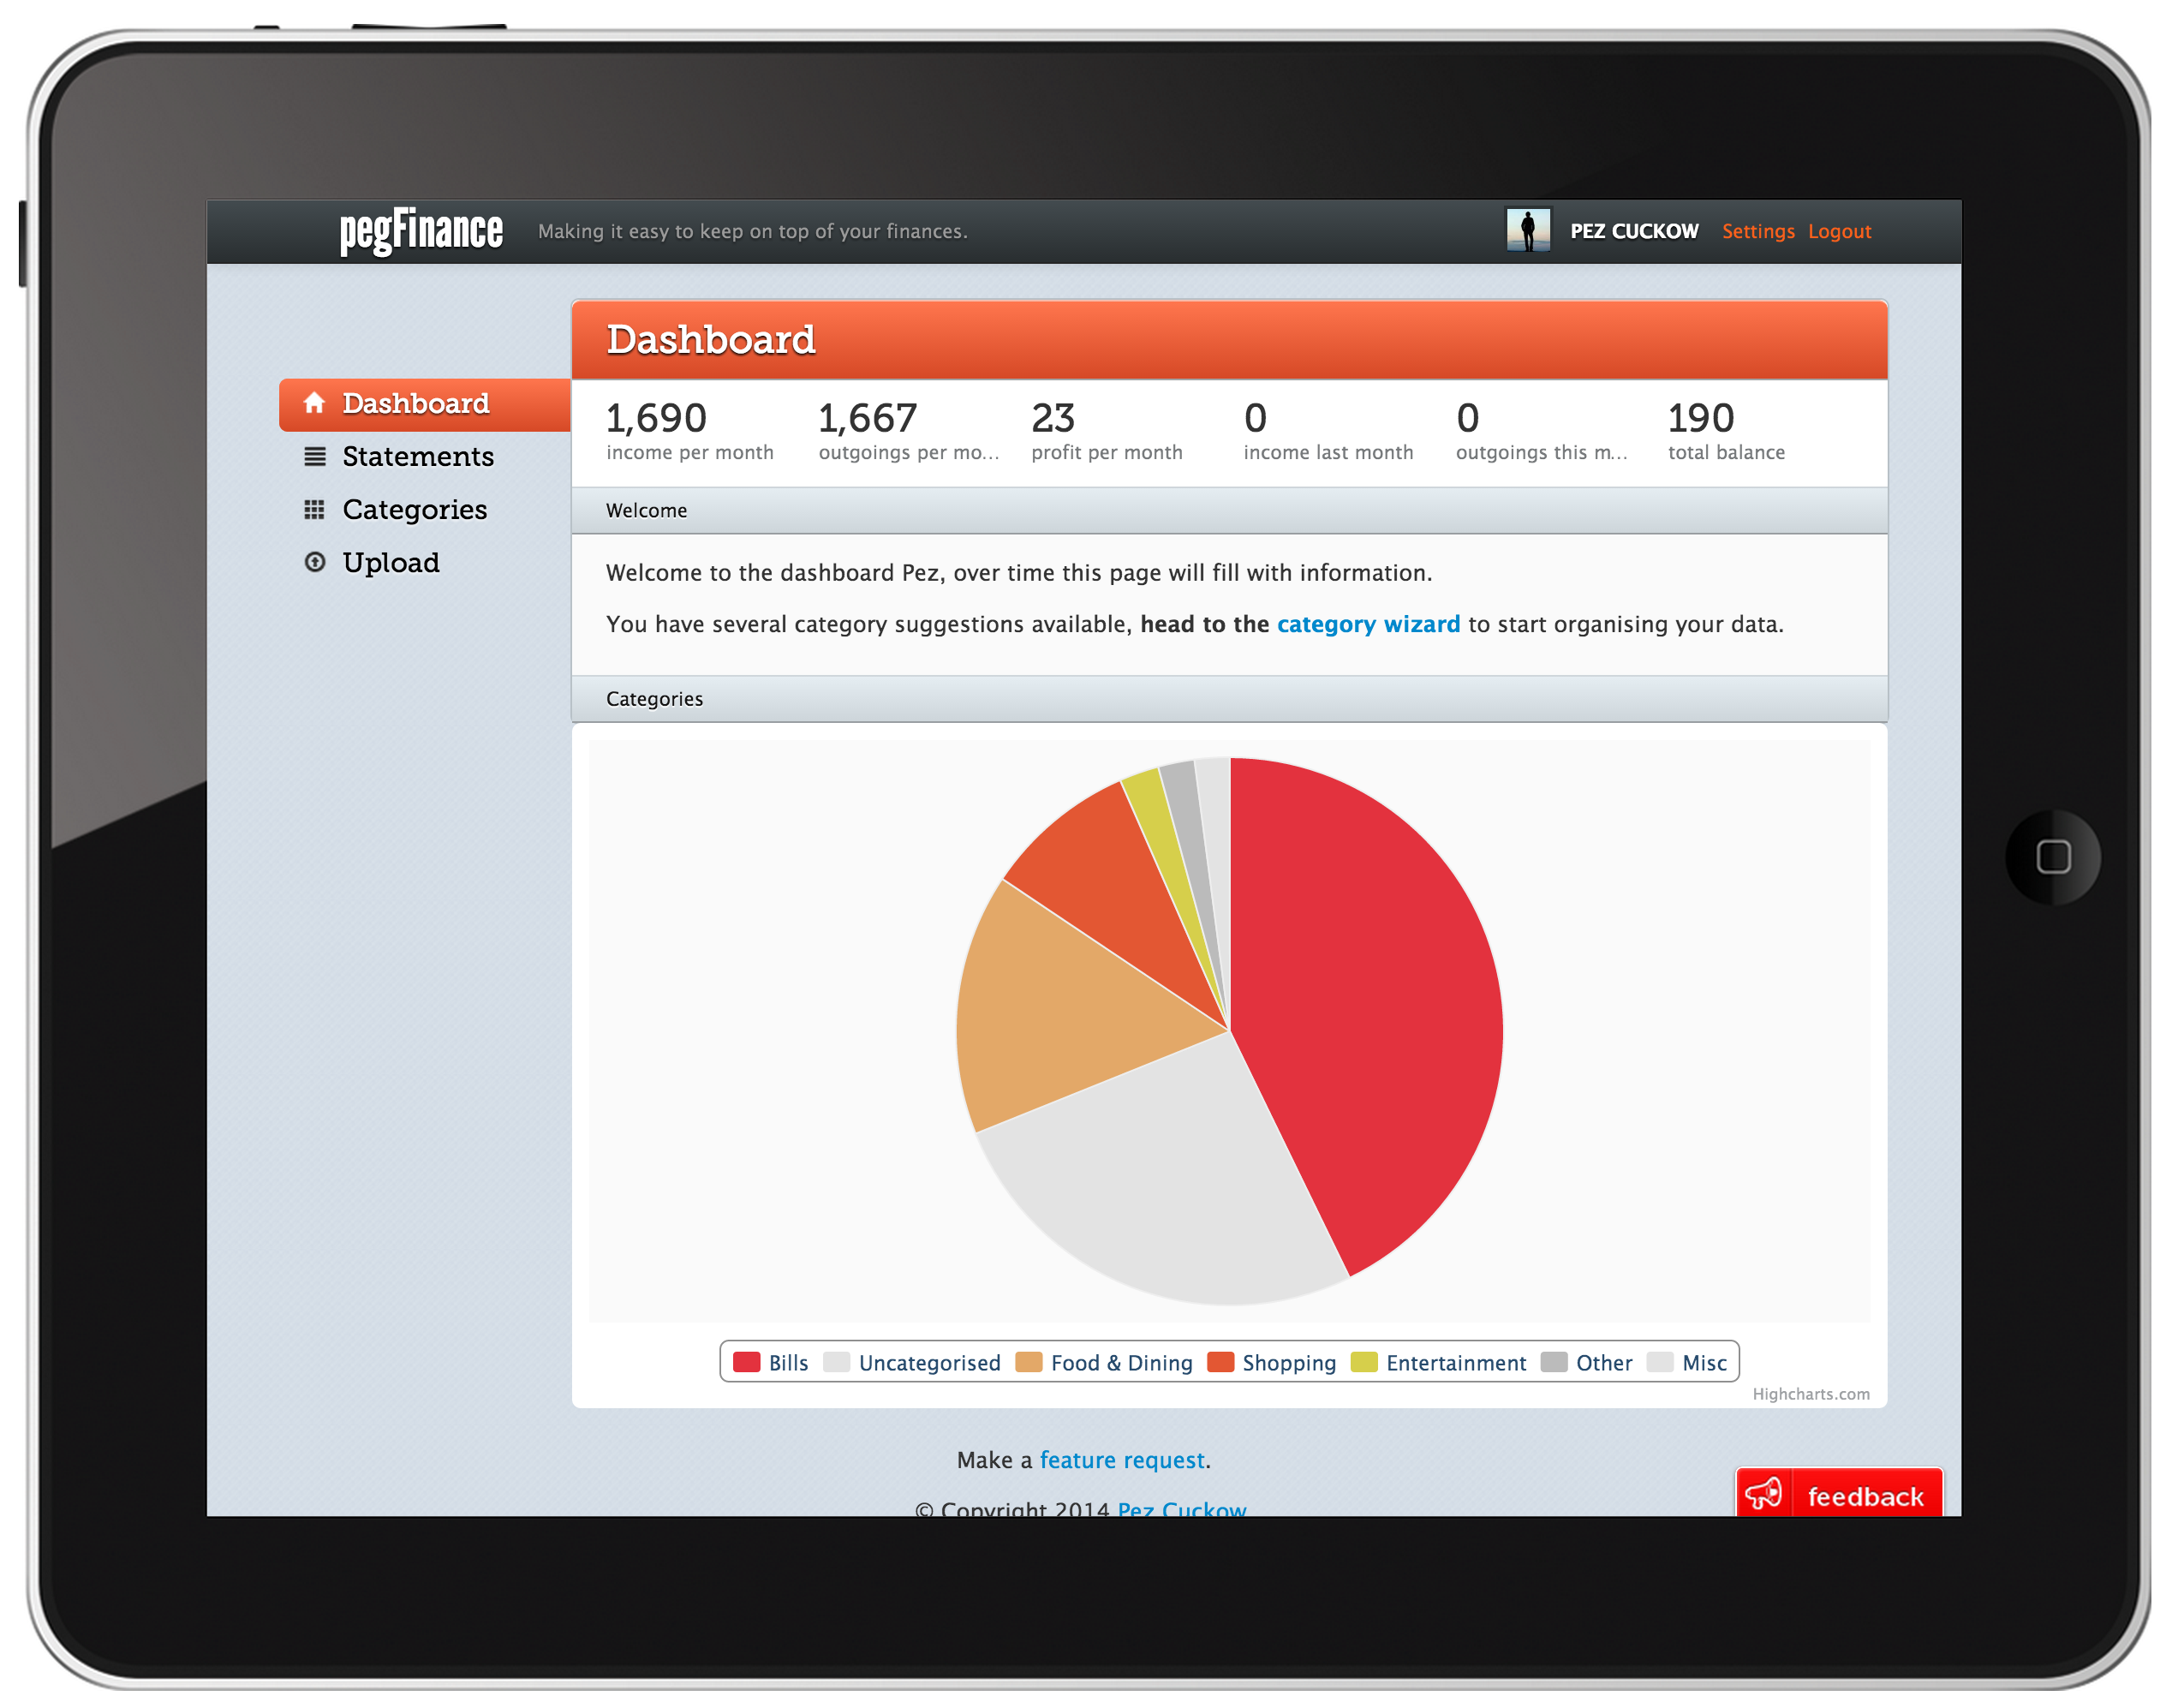
\includegraphics[width=0.8\textwidth]{screenshots/responsive/ipad-sideways}
    \caption{Layout on a tablet in landscape}
    \label{fig:responsive-ipad}
\end{figure}

\begin{figure}[h]
    \centering
    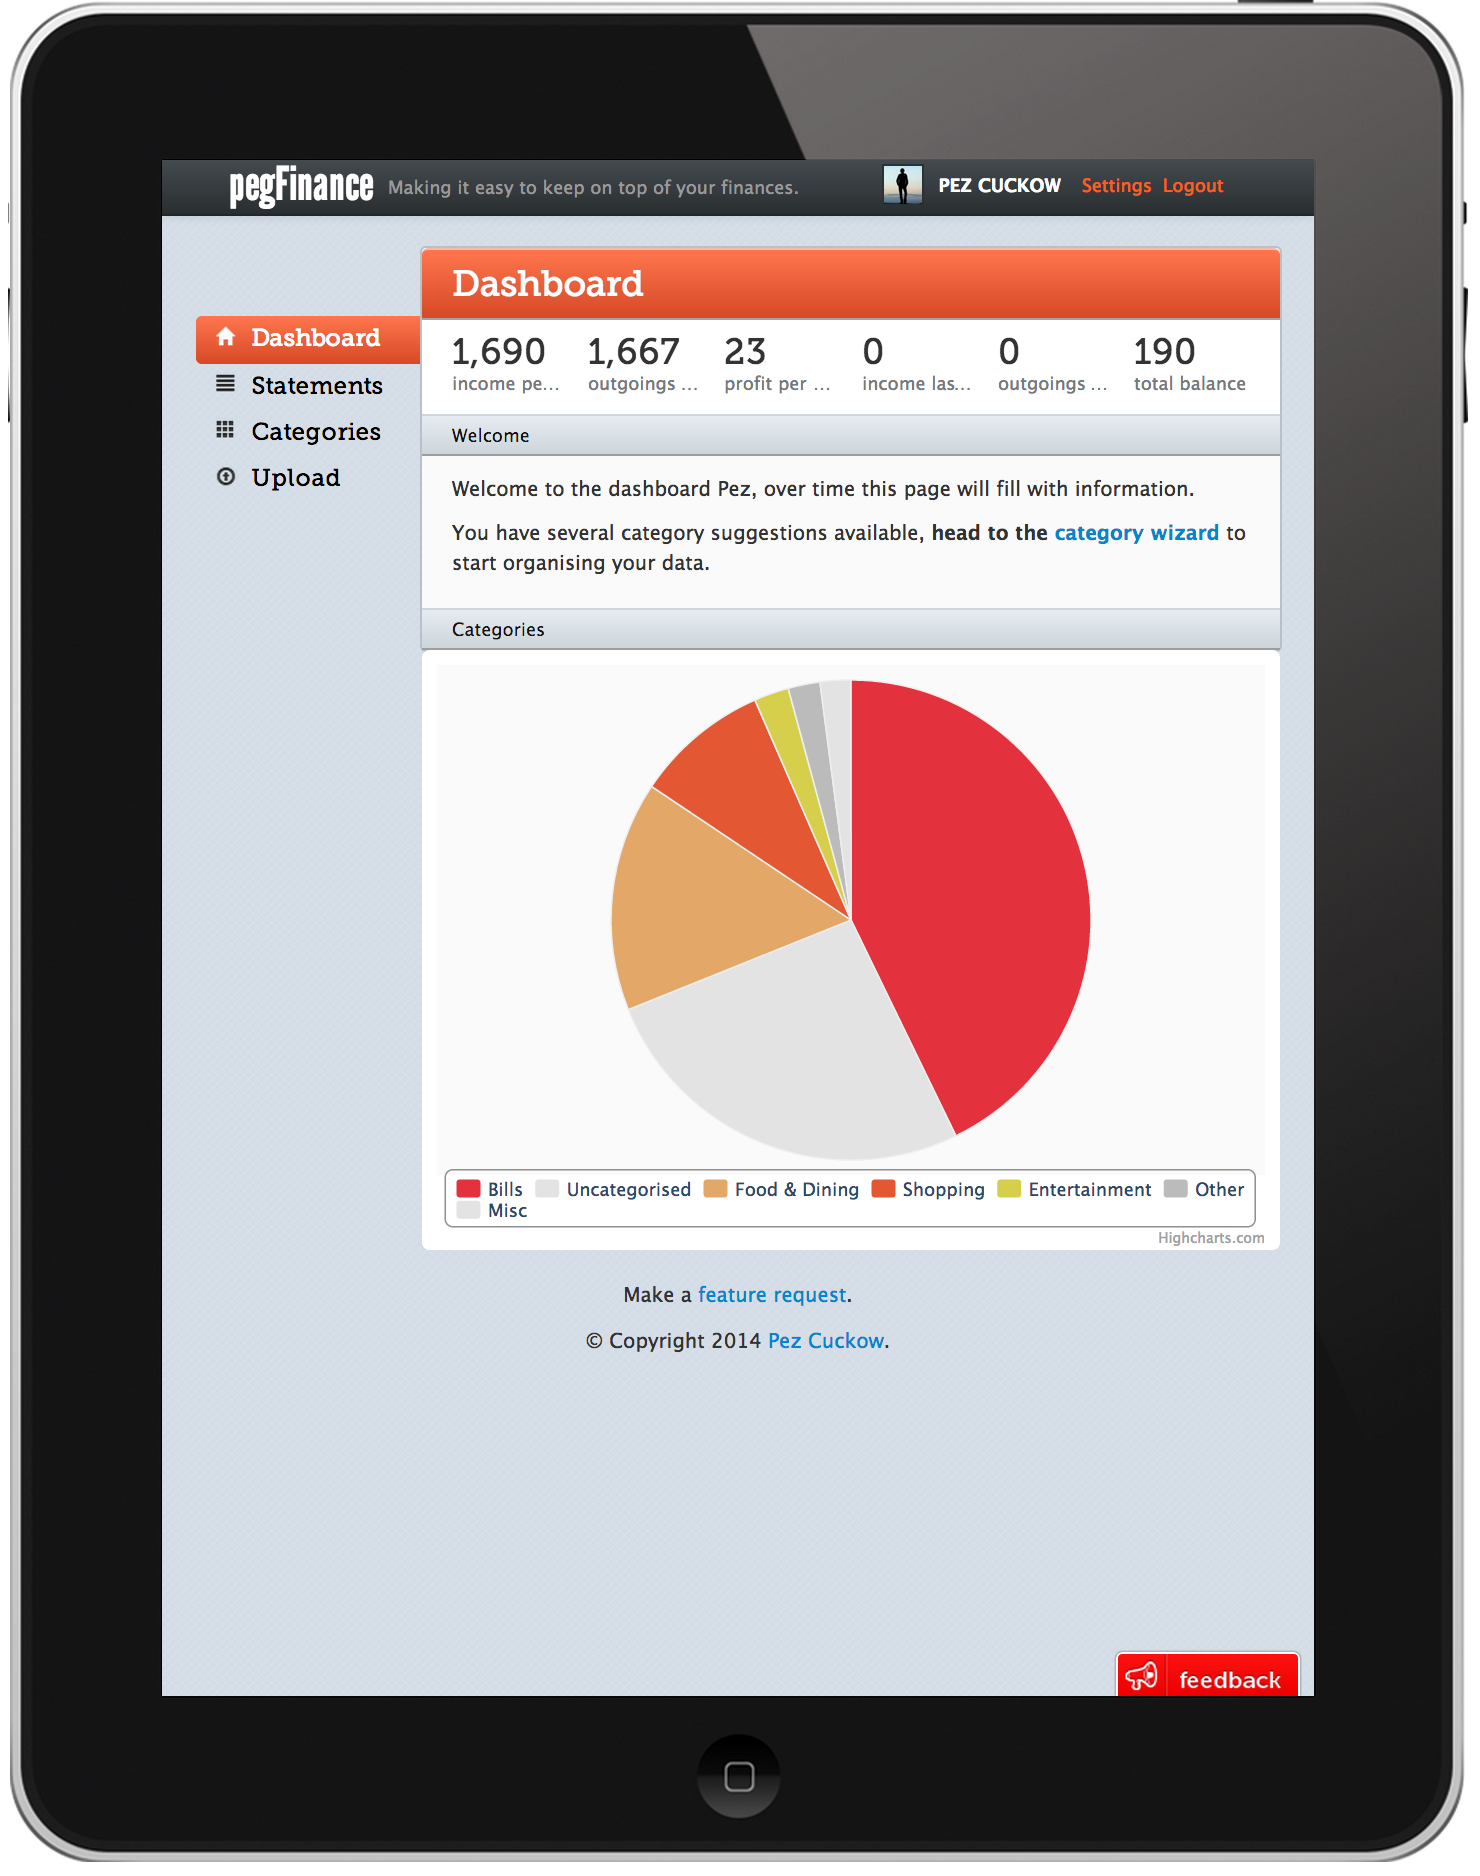
\includegraphics[width=0.5\textwidth]{screenshots/responsive/ipad-portrait}
    \caption{Layout on a tablet in portrait}
    \label{fig:responsive-ipad2}
\end{figure}

\begin{figure}[h]
    \centering
    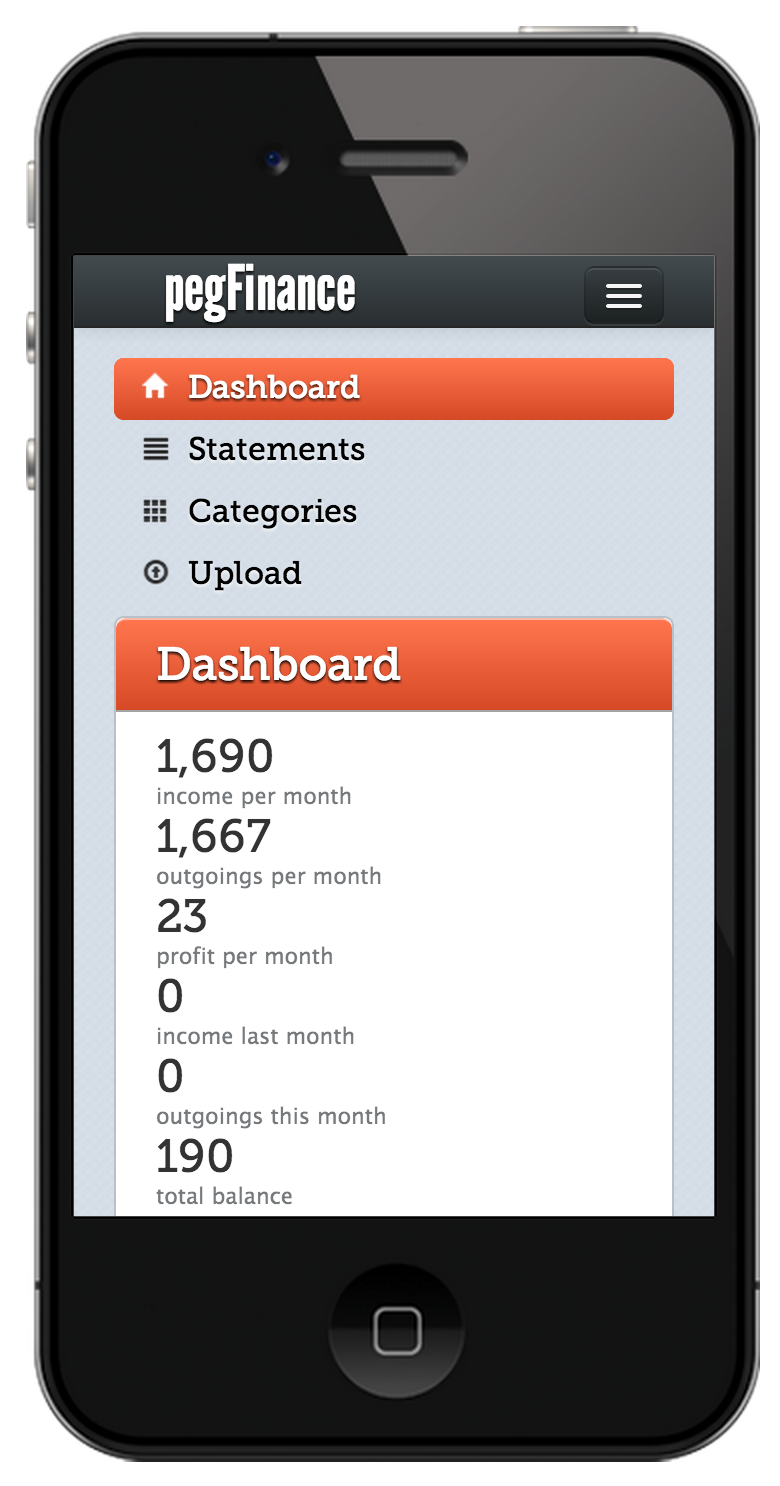
\includegraphics[width=0.5\textwidth]{screenshots/responsive/iphone-portrait}
    \caption{Layout on a smaller smartphone}
    \label{fig:responsive-iphone}
\end{figure}

%\section{Uploading a Statement}

%\section{Suggestion Engine}

%\section{Viewing Statements}

%\section{Prediction Overview}